% This LaTeX was auto-generated from MATLAB code.
% To make changes, update the MATLAB code and export to LaTeX again.

\documentclass{article}

\usepackage[utf8]{inputenc}
\usepackage[T1]{fontenc}
\usepackage{lmodern}
\usepackage{graphicx}
\usepackage{color}
\usepackage{hyperref}
\usepackage{amsmath}
\usepackage{amsfonts}
\usepackage{epstopdf}
\usepackage[table]{xcolor}
\usepackage{matlab}

\sloppy
\epstopdfsetup{outdir=./}
\graphicspath{ {./solar-house_images/} }

\matlabmultipletitles

\begin{document}

\matlabtitle{\textbf{Modeling of Passive Solar House in Boston, MA}}

\begin{par}
\begin{center}
\textbf{Nathan Faber and Jack Greenberg | October 2020}
\end{center}
\end{par}

\matlabheading{\textbf{I}ntroduction and Background}

\matlabheadingthree{What is a passive solar home?}

\begin{par}
\begin{flushleft}
Passive solar houses are incredible. By definition passive solar houses they use energy from the sun and their surroundings to maintain a livable internal temperature. Everyone should be interested in building one as passive homes are much cheaper to heat and cool since they are designed in such a way to naturally maintain reasonable temperatures. 
\end{flushleft}
\end{par}

\begin{par}
\begin{flushleft}
Passive solar homes are built on the principle of storing energy from the sun. At a base level they require: 
\end{flushleft}
\end{par}

\begin{itemize}
\setlength{\itemsep}{-1ex}
   \item{\begin{flushleft} A large thermal mass (like stone floors) to store energy from the sun \end{flushleft}}
   \item{\begin{flushleft} Large south facing windows to collect sun, specifically in the winter months \end{flushleft}}
   \item{\begin{flushleft} Some form of insulation to reduce heat loss \end{flushleft}}
   \item{\begin{flushleft} Other controls/design choices to block sun in certain situations (eaves, trees, etc) \end{flushleft}}
\end{itemize}

\matlabheadingthree{What's our strategy?}

\begin{par}
\begin{flushleft}
Designing a passive solar house for the Boston area where it gets very cold in the winter will require careful design of the house. In attempt to maintain a stable internal temperature, our first model/design will incorporate the following features:
\end{flushleft}
\end{par}

\begin{itemize}
\setlength{\itemsep}{-1ex}
   \item{\begin{flushleft} Extremely large south facing window \end{flushleft}}
   \item{\begin{flushleft} Eaves that protect the windows/thermal mass during the summer \end{flushleft}}
   \item{\begin{flushleft} A tile floor that act's as a large thermal mass \end{flushleft}}
   \item{\begin{flushleft} No windows in any other walls \end{flushleft}}
   \item{\begin{flushleft} A very tiny floorplan (\textasciitilde{}200sqft) \end{flushleft}}
   \item{\begin{flushleft} Insulation in the ceiling, walls, and floor \end{flushleft}}
\end{itemize}


\matlabheading{Modeling}

\begin{par}
\begin{flushleft}
Our house can be simplified down to a very simple resistance network. We abstract the floor as the heat capacity for the entire house, the walls as purely insulation, and the window size as a control of the amount of energy coming into the house. Below is our resistance network modeled like a circuit.
\end{flushleft}
\end{par}

\begin{par}
\begin{center}

\includegraphics[width=\maxwidth{42.84997491219268em}]{image_0}
\end{center}
\end{par}

\matlabheadingthree{Assumptions}

\begin{par}
\begin{flushleft}
Key assumptions allow the simplification of this complex system to the above network. These include:
\end{flushleft}
\end{par}

\begin{itemize}
\setlength{\itemsep}{-1ex}
   \item{\begin{flushleft} Air doesn't enter or leave the house \end{flushleft}}
   \item{\begin{flushleft} Insulation (the walls) is purely a resistance, and doens't store any heat \end{flushleft}}
   \item{\begin{flushleft} The only heat storage is in the large thermal mass (floor) \end{flushleft}}
   \item{\begin{flushleft} Radiation only hits the window and the heat storage unit \end{flushleft}}
   \item{\begin{flushleft} All radiation through window hits the heat storage unit \end{flushleft}}
   \item{\begin{flushleft} Heat transfer and resistance is the same for all walls, floors, and ceilings of the same materials \end{flushleft}}
   \item{\begin{flushleft} Heat storage unit is at spatially uniform temperature \end{flushleft}}
\end{itemize}

\begin{par}
\begin{flushleft}
These assumptions are justified. 
\end{flushleft}
\end{par}

\begin{itemize}
\setlength{\itemsep}{-1ex}
   \item{\begin{flushleft} Air doesn't have a large thermal mass, and won't exchange much if windows etc aren't opened \end{flushleft}}
   \item{\begin{flushleft} Insulation has a much lower heat capacity than the floor \end{flushleft}}
   \item{\begin{flushleft} Radiation in Boston in winter will not change internal temp much, also very complex to implement \end{flushleft}}
   \item{\begin{flushleft} If the window is designed properly than it is possible that most of the sunlight hit's the thermal mass \end{flushleft}}
   \item{\begin{flushleft} The change in materials/properties for cieling/walls, would add complexity but would be hard to verify/produce better results \end{flushleft}}
   \item{\begin{flushleft} The floor should heat up close to uniformly. This simplifies the heat transfer more than it detracts from the accuracy of the model. It would be extremely difficult to model differently \end{flushleft}}
\end{itemize}

\matlabheadingthree{Governing  ODE's}

\begin{par}
\begin{flushleft}
The simplification of this house makes it possible to model behavior of the various parts of the house by using an Ordinary Differential Equation.
\end{flushleft}
\end{par}

\begin{par}
\begin{flushleft}
This simple house makes use of just one ODE, it describes the rate of change of the temperature of the floor ($T_{floor}$) in realtion to time. This value depends on the amount of energy coming into the floor via solar radiation ($Q_{in}$). The floor also loses energy to its surroundings through the air and then the walls. This rate is influenced by the temperature differential between the outside and inside air and the overall resistance that is calculated from the geometry and materials of the house.
\end{flushleft}
\end{par}

\begin{par}
\begin{flushleft}
\textit{ODE describing rate of change of the Temp of the floor}
\end{flushleft}
\end{par}

\begin{par}
$$\frac{dT_{floor} }{dt}=\frac{Q_{in} }{C_{floor} }-\frac{T_{floor} -T_{out} }{C_{floor} \cdot R_{total} }$$
\end{par}

\begin{par}
\begin{flushleft}
When designing a passive solar house, one of the most important things to look at is the internal air temperature. The inside air temperature can be modeled as a linear function of the floor temperature.
\end{flushleft}
\end{par}

\begin{par}
\begin{flushleft}
\textit{Realtionship between the Temp of the air inside the house and the floor}
\end{flushleft}
\end{par}

\begin{par}
$$T_{inside~air} =\frac{R_{parallel} }{R_{total} }\cdot T_{floor}$$ 
\end{par}

\matlabheadingtwo{Parameters}

\matlabheadingthree{Time}

\begin{par}
\hfill \break
\end{par}

\begin{matlabcode}
% Number of days to run the model
days = 14;

% Timespan for the model
step_size = 60;
time_span = [0:step_size:60*60*24*days];
\end{matlabcode}

\matlabheadingthree{Dimensions}

\begin{par}
\begin{flushleft}
A helper function is used to calculate all of the different parameters of the house.
\end{flushleft}
\end{par}

\begin{par}
\begin{flushleft}
The final parameters we used are a floor thickness of 0.275 meters, an insulation thickness of 5.125cm, and a window border of 0.5m (amount of space on either side of the window made of insulation).
\end{flushleft}
\end{par}

\begin{matlabcode}
[house insulation floor window R outside_air inside_air, Qin] = calculate_constants(0.275,.05125,0.5) %Floor Thick, Insul Thick, Window border(larger number makes window smaller)
\end{matlabcode}
\begin{matlaboutput}
house = 
                        x: 5
                        y: 3
                        z: 5
                    sq_ft: 269.0975
                     eave: 0.9000
       ceiling_floor_area: 25
           side_wall_area: 15
    anti_window_wall_area: 15
         window_wall_area: 6

insulation = 
     thickness: 0.0512
             k: 0.0400
    total_area: 101

floor = 
            x: 5
            z: 5
            y: 0.2750
      density: 3000
    spec_heat: 800
         mass: 20625
          T_0: 0
           sa: 55.5000
      heat_in: []
     heat_cap: 16500000

window = 
           h: 0.7000
           y: 2
           z: 4.5000
        area: 9
    y_offset: 0.2000

R = 
          air_wall: 6.6007e-04
              wall: 0.0127
      wall_outside: 3.3003e-04
        wall_total: 0.0137
        air_window: 0.0074
            window: 0.1587
    window_outside: 0.0037
      window_total: 0.1698
              loss: 0.0127
         floor_air: 0.0012
             total: 0.0139

outside_air = 
      T: -3
      h: 30
    sin: @(t)(-3+6*sin((2*pi*t)/(24*60*60)+(3*pi)/4))

inside_air = 
    T_0: 0
      h: 15

Qin = 
    @(t)(-361*cos((pi*t)/(12*3600))+224*cos((pi*t)/(6*3600))+210)*window.area

\end{matlaboutput}


\matlabheadingtwo{ODEs and other Relationships}

\begin{par}
\begin{flushleft}
\textit{ODE describing rate of change of the Temp of the floor}
\end{flushleft}
\end{par}

\begin{par}
$$\frac{dT_{floor} }{dt}=\frac{Q_{in} }{C_{floor} }-\frac{T_{floor} -T_{out} }{C_{floor} \cdot R_{total} }$$
\end{par}

\begin{par}
\begin{flushleft}
\textit{Relationship describing rate of change of the Temp of the air inside the house}
\end{flushleft}
\end{par}

\begin{par}
$$T_{inside~air} =\frac{R_{parallel} }{R_{total} }\cdot T_{floor}$$ 
\end{par}

\matlabheadingtwo{First pass model with constant outside temperature}

\begin{matlabcode}
% Set up and solve ODEs
f = @(t,T) Qin(t)/floor.heat_cap - (T(1)-outside_air.T)/(R.total*floor.heat_cap);
[t,T_sol] = ode45(f,time_span,[0]);

% Compute inside air temperature using voltage divider analogy
T_sol(:,2) = T_sol(:, 1) * (R.loss/R.total);

% Plot
figure
plot_ode(t, T_sol, true)
\end{matlabcode}
\begin{matlaboutput}
Warning: MATLAB has disabled some advanced graphics rendering features by switching to software OpenGL. For more information, click here.
\end{matlaboutput}
\begin{matlabcode}
final_touches_plot()
title("Temperature of house through 2 weeks (Constant air temp -3^{\circ}C)")
\end{matlabcode}
\begin{center}
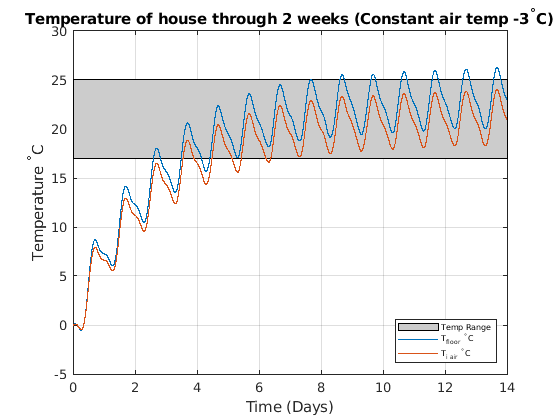
\includegraphics[width=\maxwidth{56.196688409433015em}]{figure_0.png}
\end{center}


\matlabheadingtwo{Second pass model with outside temperature as a sin function}

\begin{matlabcode}
% Set up and solve ODEs
f = @(t,T) Qin(t)/floor.heat_cap - (T(1)-outside_air.sin(t))/(R.total*floor.heat_cap);
[t_sin,T_sol_sin] = ode45(f,time_span,[0]);

% Compute inside air temperature using voltage divider analogy
T_sol_sin(:,2) = T_sol_sin(:, 1) * (R.loss/R.total);
\end{matlabcode}


\begin{matlabcode}
figure
plot_ode(t_sin, T_sol_sin, true)
final_touches_plot()
title("Temperature of house through 2 weeks (Outside air Sin function) ")
\end{matlabcode}
\begin{center}
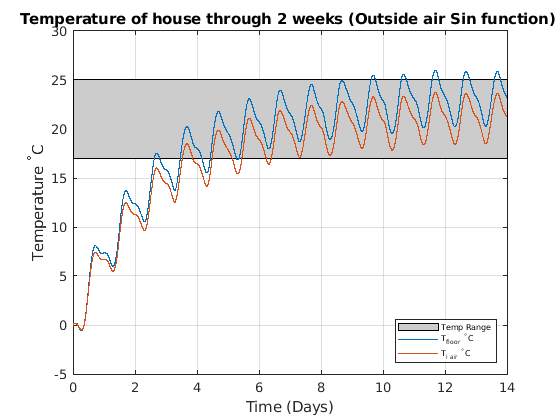
\includegraphics[width=\maxwidth{56.196688409433015em}]{figure_1.png}
\end{center}

\begin{par}
\begin{flushleft}
The above plot shows the house's temperature as a function of time. The shaded region represents the desired range of temperature for a day. The house takes several days to warm up before it stables in a region within our desired range of 17-25. These reults are obtained by using Matlab's ode45 solver to solve our differential equation.
\end{flushleft}
\end{par}


\matlabheadingtwo{Optimization}

\begin{matlabcode}
values = 5;
min_insul = 0.045;
max_insul = 0.07;
min_floor_thick = 0.15;
max_floor_thick = 0.4;
min_win = 1;
max_win = 0;% Window is ntire width of house
insul_range = linspace(min_insul, max_insul, values);
floor_range = linspace(min_floor_thick, max_floor_thick, values);
win_range = linspace(min_win, max_win, 3);

plot_num = 1;
x = linspace(0,10);
figure1=figure('Position', [100, 100, 4000, 4000]);
for i = insul_range
    for k = floor_range
        %Set appropriate values
        subplot(values,values,plot_num)
        for w = win_range
            [house insulation floor window R outside_air inside_air, Qin] = calculate_constants(k, i, w);
            f = @(t,T) [Qin(t)/floor.heat_cap - (T(1)-outside_air.sin(t))/(R.total*floor.heat_cap);];
            [t_sin,T_sol_sin] = ode45(f,time_span,[0]);
            T_sol_sin(:,2) = T_sol_sin(:, 1) * (R.loss/R.total); % Use voltage divider analogy to calculate internal air temp    
            plot_ode(t_sin, T_sol_sin, false, window.area)
        end
        final_touches_plot(true)
        title( k + "m floor, " + i + "m insul")
        
%         
%         y1 = 10*i*sin(x)+k;
%         plot(x,y1)
%         title("Subplot"+ plot_num + ": sin(x)")
        plot_num = plot_num + 1;
    end
    
end
han=axes(figure1,'visible','off'); 
han.Legend;
\end{matlabcode}
\begin{matlaboutput}
ans = 
  0x0 empty GraphicsPlaceholder array.

\end{matlaboutput}
\begin{matlabcode}
han.Title.Visible='on';
han.XLabel.Visible='on';
han.YLabel.Visible='on';
xlabel("Time (Days)");
ylabel("Temperature ^{\circ}C");
\end{matlabcode}

\matlabheadingtwo{Sweep of various floor and insulation thicknesses with different window sizes}

\begin{par}
\begin{center}
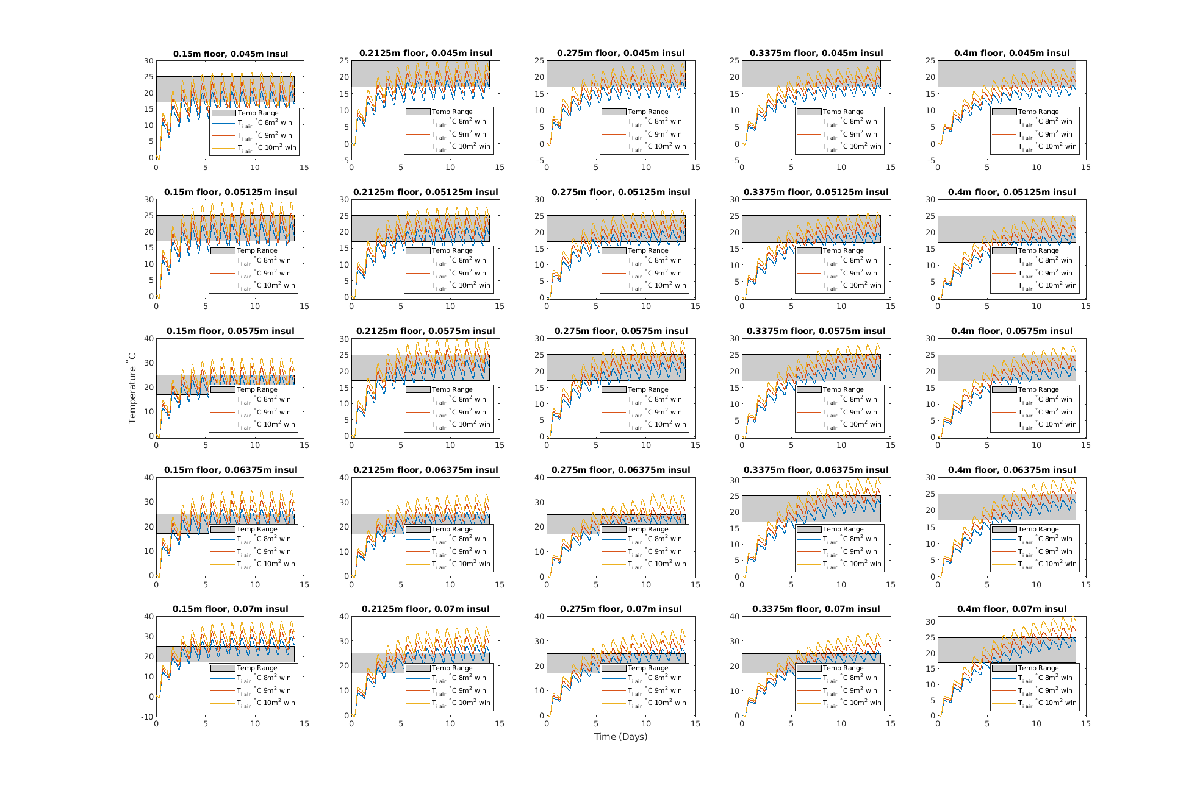
\includegraphics[width=\maxwidth{120.42147516307075em}]{image_1}
\end{center}
\end{par}

\begin{par}
\begin{flushleft}
From the results above we can see that insulation thickness and floor thickness both change the temperature profile of our house.
\end{flushleft}
\end{par}

\begin{par}
\begin{flushleft}
As floor thickness increases the time it takes to reach a consistent periodic temperature increases. This is due to the increase in thermal mass, hence more energy is needed to "charge" the floor (imagine the floor as a heat capacitor). The increased thermal mass also reduces the amplitude of the temperature fluctuation throughtout the day. This is because the larger floor acts like a larger capacitor, hence smoothing out the changes in heat transfer due to changing solar radiation. 
\end{flushleft}
\end{par}

\begin{par}
\begin{flushleft}
Increases in insulation thickness have the effect of increasing the average daily temperature after steady state has been reached. This is due to the fact that the same amount of energy is being added, but the amount of thermal resistance is increasing, thus effectively trapping more heat within the house. Interestingly, we also see that the change in insulation thickness has no significant on the amplitude of the daily temperature fluctuations at steady state.
\end{flushleft}
\end{par}

\begin{par}
\begin{flushleft}
The final value we swept was the window size. As should be apparent by the chart, we can see that larger windows lead to higher heat, which makes intuitive sense because there will be more solar radiation entering into the house. While the changes in window size appear to have a linear effect on average daily temperature, this is likely due to the fact that the model uses a "perfect" window, and doesn't account for any thermal storage or light reflection from the sun.
\end{flushleft}
\end{par}


\matlabheadingtwo{Results and discussion}

\matlabheadingthree{Single day}

\begin{par}
\hfill \break
\end{par}

\begin{matlabcode}
% Fetch the constants we used in our final model once more
[house insulation floor window R outside_air inside_air, Qin] = calculate_constants(0.275,.05125,0.5);

% Re-set up and solve ODEs
f = @(t,T) [Qin(t)/floor.heat_cap - (T(1)-outside_air.sin(t))/(R.total*floor.heat_cap);];
[t_sin,T_sol_sin] = ode45(f,time_span,[0]);

% Re-compute inside air temperature using voltage divider analogy
T_sol_sin(:,2) = T_sol_sin(:, 1) * (R.loss/R.total);

day_start = 12;
day_end = 13;
day_ticks = ["12am","6am","12pm","6pm",];
seconds_in_day = 24*3600/step_size;
day_start_index = 1+day_start*seconds_in_day;
day_end_index = day_end*seconds_in_day;

figure
% plot(t_sin(day_start_index:day_end_index,:)/(60*60*24), T_sol_sin(day_start_index:day_end_index,1), "DisplayName", "T_{floor} ^{\circ}C");
hold on;
plot(t_sin(day_start_index:day_end_index,:)/(60*60*24), T_sol_sin(day_start_index:day_end_index,2), "DisplayName", "T_{inside air} ^{\circ}C");

[maxVal,maxIDX] = max(T_sol_sin(day_start_index:day_end_index,2));
[minVal,minIDX] = min(T_sol_sin(day_start_index:day_end_index,2));
% % % for single point plotting, use scatter
scatter((t_sin(day_start_index+maxIDX))/(60*60*24), maxVal, '*r', "DisplayName", "Max T ^{\circ}C")
scatter((t_sin(day_start_index+minIDX))/(60*60*24), minVal, '*b', "DisplayName", "Min T ^{\circ}C")

dx = 0.05; dy = 0.05; % displacement so the text does not overlay the data points
text((t_sin(day_start_index+maxIDX))/(60*60*24)+dx, maxVal+dy, "Max is: "+ maxVal + "^{\circ}C");
text((t_sin(day_start_index+minIDX))/(60*60*24)+dx, minVal+dy, "Min is: "+ minVal + "^{\circ}C");

final_touches_plot
xticks(day_start:1/4:day_end)
xticklabels(repmat(day_ticks, 1, day_end-day_start));
ylim([16 26])
title("Temperature of house on days " + day_start + " - " + day_end)
\end{matlabcode}
\begin{center}
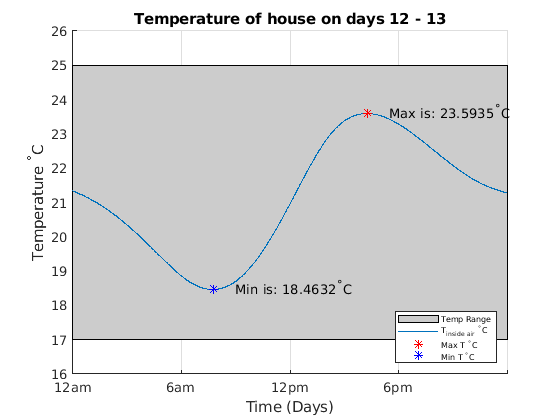
\includegraphics[width=\maxwidth{56.196688409433015em}]{figure_2.png}
\end{center}

\begin{par}
\begin{flushleft}
This house's temperature fluctuates roughly $5^{\circ } C$throughout the day. This is slightly larger than the average house, which typically ranges from $20-22^{\circ } C$ (1). This simply means that our house changes temperature more than a typical house. A person living in this house would likely experience some discomfort since at various point in the day they would want to switch from wearing a sweater or jacket to just a t-shirt to maintain a comfortable body temperature.
\end{flushleft}
\end{par}

\begin{par}
\begin{flushleft}
Since we still have a fairly high temperature fluctuation, and as we can see from the optimization grid, adding more thermal mass to the house would likely decrease the range in temperature and make living more comfortable. For instance, adding a large fish tank would allow the temperature to absorb some of the heat, although may be less comfortable for the fish.
\end{flushleft}
\end{par}


\matlabheadingtwo{Analyzing heat absorbed through the window for one day and temperature change}

\begin{par}
\begin{flushleft}
We were concerned with how hot our floor/house was getting (\textasciitilde{}60*C). To take a look at possible explanations for this behavior we wanted to look at how much energy was coming into the house. 
\end{flushleft}
\end{par}

\begin{par}
$$Q_{in} =(-361\cdot \cos (\frac{t\pi }{12\cdot 3600})+224\cdot \cos (\frac{t\pi }{6\cdot 3600})+210)\cdot A_{window.area}$$
\end{par}

\begin{matlabcode}
% Calculate and plot the solar heat and outside air temp for one day
one_day = [0 : 60*60 : 24*3600]; % Calculated each hour
solar_day = Qin(one_day);
out_air = outside_air.sin(one_day);

figure
plot(one_day/3600, solar_day, "DisplayName", "Qin (Solar) W");
yyaxis right
plot(one_day/3600, out_air , "DisplayName", "T_{outside air} ^{\circ}C");
xticks([0,6,12,18,24]);
xticklabels([["Midnight","6am","Noon","6pm","Midnight"]])
grid on; legend("Location", "Southeast");
xlabel("Time of Day")
ylabel("Air Temp ^{\circ}C")
yyaxis left
ylabel("Heat absorbed (Watts)")
title("Heat absorbed through " + window.area + "m^2 window throughout day")
\end{matlabcode}
\begin{center}
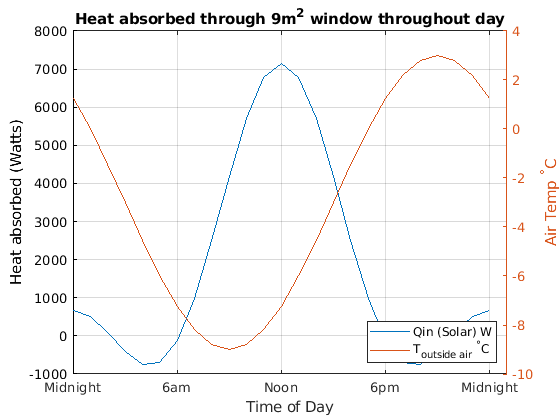
\includegraphics[width=\maxwidth{56.196688409433015em}]{figure_3.png}
\end{center}

\begin{par}
\begin{flushleft}
This plot shows the amount of energy coming into the house at various points of the day for our given window size. It also shows the outside temperature of the house throughout the day. Together, these curves explain the shape of the floor temperature curve seen in one day.
\end{flushleft}
\end{par}


\vspace{1em}
\begin{par}
\begin{flushleft}
At it's peak, there is \textasciitilde{}10,000 watts coming into the house. This value seemed really high at first! However, according to some sources, this is likely realistic. Tennessee Solar info indicates that at the surface of the earth in good conditions solar flux could be around \textasciitilde{}1000 w/m\textasciicircum{}2. Our window is 13m\textasciicircum{}2 which indicates that our max solar flux is \textless{} 1000W/m\textasciicircum{}2 and is likely within an acceptable range.
\end{flushleft}
\end{par}

\matlabheading{Extensions}

\begin{par}
\begin{flushleft}
If we had had more time, there are a number of project extensions we had considered. It would have been interesting to programmatically calculate the best values for our parameters. These parameters would heat up the house quickly initially, and keep the temperature within our range of values with smaller fluctuations throughout the day. We could accomplish this using a gradient descent model, where our reward function is the min and max temperature or cost of building materials, the goal would be to keep it in the 18-25 degree celcius range with minimal fluctuations, and using reasonable domains to ensure a plausible design (for example, so that we don't get a 10 kilometer thick floor).
\end{flushleft}
\end{par}


\vspace{1em}
\matlabheading{Bibliography}

\begin{par}
\begin{flushleft}
“Room Temperature.” \textit{Wikipedia}, Wikimedia Foundation, 29 Sept. 2020, 
\end{flushleft}
\end{par}

\begin{par}
\begin{flushleft}
    \href{http://“Room Temperature.” Wikipedia, Wikimedia Foundation, 29 Sept. 2020, en.wikipedia.org/wiki/Room_temperature. }{en.wikipedia.org/wiki/Room\_temperature. }
\end{flushleft}
\end{par}

\begin{par}
\begin{flushleft}
“Guide to Passive Solar Home Design.” \textit{Energy Efficiency and Renewable Energy}, United States Department of Energy, Oct. 2010,
\end{flushleft}
\end{par}

\begin{par}
\begin{flushleft}
    \href{www.energy.gov/sites/prod/files/guide_to_passive_solar_home_design.pdf.}{www.energy.gov/sites/prod/files/guide\_to\_passive\_solar\_home\_design.pdf.}
\end{flushleft}
\end{par}

\begin{par}
\begin{flushleft}
“The Sun's Energy.” \textit{Solar and Sustainale Energy}, 
\end{flushleft}
\end{par}

\begin{par}
\begin{flushleft}
    \href{https://ag.tennessee.edu/solar/Pages/What%20Is%20Solar%20Energy/Sun%27s%20Energy.aspx}{ag.tennessee.edu/solar/Pages/What\%20Is\%20Solar\%20Energy/Sun\%27s\%20Energy.aspx. }
\end{flushleft}
\end{par}

\begin{par}
\begin{flushleft}
“Passive Solar Home Design.” \textit{Energy.gov}, 
\end{flushleft}
\end{par}

\begin{par}
\begin{flushleft}
    \href{http://www.energy.gov/energysaver/energy-efficient-home-design/passive-solar-home-design. }{www.energy.gov/energysaver/energy-efficient-home-design/passive-solar-home-design. }
\end{flushleft}
\end{par}


\matlabtitle{Functions, Constants, and Code}

\begin{matlabcode}
function a = plot_ode(x,y, both, win_area)
    if nargin<4
        % Then no window area was supplied
        text = "";
    else
        text = win_area + "m^2 win";
    end
    
    if both 
        plot(x/(60*60*24), y(:,1), "DisplayName", "T_{floor} ^{\circ}C " + text);
        hold on;
    end
    plot(x/(60*60*24), y(:,2), "DisplayName", "T_{i air} ^{\circ}C " + text);
    hold on
end
function a = final_touches_plot(noaxis)
    if nargin<1
        % Then no window area was supplied
        noaxis = false;
    end
    ybars = [17 25];
    p = patch([min(xlim) max(xlim) max(xlim) min(xlim)], [ybars(1) ybars(1), ybars(2) ybars(2)], [0.8 0.8 0.8], "DisplayName", "Temp Range");
    uistack(p, "bottom");
    if noaxis
        
    else
       add_axis
    end
    add_legend
    hold off
end

function a = add_axis()
    grid on;     
    xlabel("Time (Days)");
    ylabel("Temperature ^{\circ}C");
end
function a = add_legend()
    lgd = legend("Location", "Southeast");
    lgd.FontSize = 6;
end

function [house, insulation, floor, window, R, outside_air, inside_air, Qin] = calculate_constants(floor_thick, insul_thick, window_offset)
    if nargin<3
      floor_thick = 0.275;
      insul_thick = 0.0575;
      window_offset = 0.5;
    end
    global time_span
    % Internal dimensions of inside air
    house.x = 5.0; % meters
    house.y = 3.0; % meters
    house.z = 5.0; % meters
    house.sq_ft = house.x * house.z * 10.7639; % ft^2
    house.eave = 0.9; % m % Length of the eave of the house
    
    % Window
    window.h = 0.7;
    window.y = 2.0; % m;
    window.z = house.z-window_offset; % m % Window has a half meter wall on either side
    window.area = window.y * window.z; % m^2
    window.y_offset = 0.2; % m % Height off the ground
    
    % Floor
    floor.x = house.x;
    floor.z = house.z;
    % PARAM %
    floor.y = floor_thick; % meters
    floor.density = 3000.0; % kg/m^3
    floor.spec_heat = 800.0; % J/kg*K
    floor.mass = floor.x * floor.y * floor.z * floor.density; % kg
    floor.T_0 = 0; % C
    floor.sa = 2*floor.x*floor.y + 2*floor.x*floor.z + 2*floor.y*floor.z; % m^2 % Surface area
    
    % Walls
    house.ceiling_floor_area = house.z * house.x; % m^2
    house.side_wall_area = house.x * house.y; % m^2
    house.anti_window_wall_area = house.z * house.y; % m^2 % Wall opposite window
    house.window_wall_area = house.anti_window_wall_area - (window.area); % m^2 % WHY DO WE NEED THIS LAST PART??
    
    % PARAM %
    insulation.thickness = insul_thick; % meters
    insulation.k = 0.04; % W/m*K % Thermal conductivity constant
    insulation.total_area = 2*house.ceiling_floor_area + 2*house.side_wall_area + house.anti_window_wall_area + house.window_wall_area; % m^2
\end{matlabcode}

\matlabheadingthree{Air Temperature}

\begin{par}
\hfill \break
\end{par}

\begin{matlabcode}
    outside_air.T = -3; % degrees celcius
    outside_air.h = 30.0; % W/m^2*K
\end{matlabcode}

\begin{par}
$$T_{outside~air} =-3+6\cdot \sin (\frac{2\pi t}{24\cdot 60\cdot 60})+\frac{3\pi }{4}$$
\end{par}

\begin{matlabcode}
    outside_air.sin = @(t) (-3 + 6*sin((2*pi*t)/(24*60*60) + (3*pi)/4)); % Degrees celcius
    
    inside_air.T_0 = 0; % degrees celcius
    inside_air.h = 15.0; % W/m^2*K
\end{matlabcode}

\matlabheadingthree{Heat}

\begin{par}
\hfill \break
\end{par}

\begin{matlabcode}
    % W/m^2
    solar_flux = -361 .* cos((pi.*time_span)./(12*3600)) + 224 .* cos((pi.*time_span)./(6*3600)) + 210;
    floor.heat_in = solar_flux .* window.area; % W
    Qin = @(t) (-361 * cos((pi*t)/(12*3600)) + 224 * cos((pi*t)/(6*3600)) + 210) * window.area;
\end{matlabcode}

\matlabheadingtwo{Resistances/Capacities}

\begin{matlabcode}
    floor.heat_cap = floor.spec_heat * floor.mass; % J/K
    
    % Resistance through all the insulation
    R.air_wall = (inside_air.h * insulation.total_area)^-1; % Convection, K/W
    R.wall = insulation.thickness / (insulation.k * insulation.total_area); % Conduction, K/W
    R.wall_outside = (outside_air.h * insulation.total_area)^-1; % Convection, K/W
    R.wall_total = R.air_wall + R.wall + R.wall_outside; % K/W
    
    % Resistance through the window
    R.air_window = (inside_air.h * window.area)^-1; % Convection, K/W
    R.window = (window.h * window.area)^-1; % Conduction, K/W
    R.window_outside = (outside_air.h * window.area)^-1; % Convection, K/W
    R.window_total = R.air_window + R.window + R.window_outside; % K/W
    
    R.loss = (sum([R.wall_total R.window_total].^-1))^-1;
    
    R.floor_air = (inside_air.h*floor.sa)^-1; % Resistance from floor to inside air
    
    R.total = R.floor_air + R.loss; % Total resistance from floor to outside air
end
\end{matlabcode}

\end{document}
